\documentclass[compress, aspectratio=32]{beamer}
\usepackage[utf8]{inputenc}
\usepackage{graphicx} % Required for inserting images
\graphicspath{ {./images/} }
\usepackage{amsmath}
\usepackage{mathspec}
\usepackage{xeCJK}
\usepackage{multicol}
\usepackage{float}
\usepackage{soul}
\usepackage{hyperref}
\usepackage{caption}
\usepackage{subcaption}
\usepackage{ulem}

\useinnertheme{circles}
\useoutertheme[subsection=false, footline=authortitle]{miniframes}
%\usecolortheme{seagull}
\usefonttheme{structurebold}

\setmainfont{Sabon LT Pro}
\setsansfont{SF Pro Display}
%\setmathfont(Digits,Latin){Goldman Sans}
%\setmonofont{Roboto Mono}

% \AtBeginSection[]
% {
    
%   \begin{frame}[allowframebreaks]
    
%     \tableofcontents[currentsection]
    
%   \end{frame}
% }

\AtBeginSection[]
{
    
  \frame{\sectionpage}
}

% \AtBeginSubsection[]{
%     \begin{frame}[allowframebreaks]
%         \tableofcontents[currentsubsection]
%     \end{frame}
% }


\setbeamertemplate{navigation symbols}{\insertframenumber/\inserttotalframenumber}
\setbeamertemplate{title page}{
    \vbox{}
    \vfill
    \begin{beamercolorbox}[sep=8pt,left]{title}
        \usebeamerfont{title}\inserttitle\par
        \ifx\insertsubtitle\@empty
        \else
          \vskip0.25em
          {\usebeamerfont{subtitle}\usebeamercolor[fg]{subtitle}\insertsubtitle\par}%
        \fi     
      \end{beamercolorbox}
    \vskip1em\par
    \begin{beamercolorbox}[sep=8pt,left]{author}
      \usebeamerfont{author}\insertauthor
    \end{beamercolorbox}
    \begin{beamercolorbox}[sep=8pt,left]{institute}
        \usebeamerfont{institute}\insertinstitute
    \end{beamercolorbox}
    \begin{beamercolorbox}[sep=8pt,right]{date}
        \usebeamerfont{date}\insertdate
    \end{beamercolorbox}\vskip0.5em
    {\usebeamercolor[fg]{titlegraphic}\inserttitlegraphic\par}
    \vfill
}

\definecolor{customColor}{RGB}{163,163,163}
\setbeamercolor*{palette primary}{fg=customColor!60!black,bg=white!85!customColor}
\setbeamercolor*{palette secondary}{fg=customColor!70!black,bg=white!60!customColor}
\setbeamercolor*{palette tertiary}{bg=customColor!80!black,fg=white!50!customColor}
\setbeamercolor*{palette quaternary}{fg=customColor,bg=white!20!customColor}

\setbeamercolor*{sidebar}{fg=customColor,bg=customColor!75!white}

\setbeamercolor*{palette sidebar primary}{fg=customColor!10!black}
\setbeamercolor*{palette sidebar secondary}{fg=white}
\setbeamercolor*{palette sidebar tertiary}{fg=customColor!50!black}
\setbeamercolor*{palette sidebar quaternary}{fg=white!10!customColor}

\setbeamercolor*{titlelike}{parent=palette primary}
\setbeamercolor{frametitle}{bg=white!90!customColor}
\setbeamercolor{frametitle right}{bg=white!60!customColor}

\setbeamercolor{block title}{parent=palette tertiary}
\setbeamercolor{block body}{bg=white!90!customColor}

\setbeamercolor*{item projected}{parent=palette primary}%fg=black,bg=black!20}

\setbeamercolor*{normal text}{fg=black,bg=white}
\setbeamercolor*{alerted text}{fg=black}
\setbeamercolor*{example text}{fg=black}
\setbeamercolor*{structure}{fg=black}

\setbeamercolor{author in head/foot}{parent=title in head/foot}

\title{Ben Cheng: A Self Introduction}
\author{Po-Sheng Cheng}
\institute{RISD MID}
\date{\today}

\begin{document}

\begin{frame}
    \titlepage
\end{frame}

% \begin{frame}[allowframebreaks]{Outline}
%     \tableofcontents
% \end{frame}

\begin{frame}
    \frametitle{Ben Cheng}
    \begin{columns}
        \begin{column}{0.5\linewidth}
            \begin{itemize}
                \item Diversified interests and experiences.
                \item Strong technical skills.
                \item A good communicator.
            \end{itemize}
        \end{column}
        \begin{column}{0.5\linewidth}
            \includegraphics[width = \linewidth]{YC109980 修.jpg}
        \end{column}
    \end{columns}
\end{frame}

\section{Education}
\begin{frame}
    \frametitle{Education}
    \begin{itemize}
        \item National Taiwan University
    \begin{itemize}
        \item BSc Bio-Mechatronics Engineering
        \item BA Economics
    \end{itemize}
    \item Master of Industrial Design, Rhode Island School of Design. \begin{itemize}
        \item expected Jun. 2026
    \end{itemize} 
    \end{itemize}
    
    
\end{frame}

\begin{frame}
    \frametitle{ECE course}
    \begin{itemize}
        \item Electrical, Electronics Engineering
        \item Engineering Mathematics
              \begin{itemize}
                  \item ODE, linear algebra, fourier transform, PDE
              \end{itemize}
        \item Computer Programming Language
        \item Operating System
        \item Pratical Data Structures and Algorithms
        \item Mechatronics I-IV
              \begin{itemize}
                  \item embedded microprocessor, signal conditioning, digital circuits, system integration
              \end{itemize}
        \item BioMEMS Fabrication
        \item Intelligent Control
              \begin{itemize}
                  \item fuzzy control, genetic algorithm, neural network
              \end{itemize}
        \item Reinforcement Learning
    \end{itemize}
\end{frame}

\begin{frame}
    \frametitle{ME course}
    \begin{multicols}{2}
        \begin{itemize}
            \item Applied Mechanics I, II
            \item Strength of Materials
            \item Mechanism
            \item Design of Machine Elements
            \item Physical Chemistry
            \item Engineering Materials
            \item Fluid Mechanics
            \item Thermal Dynamics
            \item Heat Transfer
            \item Power Machinery
            \item Actuators
            \item Automatic Control
        \end{itemize}
    \end{multicols}
\end{frame}

\begin{frame}
    \frametitle{ECON course}
    \begin{multicols}{2}
        \begin{itemize}
            \item Micro
            \begin{itemize}
                \item Micro Economics I, II
                \item Game Theory
            \end{itemize}
            \item Macro
            \begin{itemize}
                \item Macro Economics I, II
                \item International Finance
                \item Trade Policy
                \item Banking and Monetary Policy
            \end{itemize}
            \item Statistics
            \begin{itemize}
                \item Introductory Statistics
                \item Introductory Econometrics
                \item Econometrics I
                \item Mathematics for Economics
            \end{itemize}
            \item Finance
            \begin{itemize}
                \item Accounting I
                \item Financial Derivatives
                \item Investment
            \end{itemize}
        \end{itemize}
    \end{multicols}
\end{frame}

\section{Experiences}

\subsection{Mechanical Engineering Intern, Logitech}
\begin{frame}
    \frametitle{Mechanical Engineering Intern, Logitech}
    \begin{itemize}
        \item Feb. 2022 - Jun 2022.
        \item Bringing electrical engineering skills to mechanical team to create new technology for keyboard.
        \item Involves ProE/Creo, R, SLA/3DP prototyping.
    \end{itemize}
    \begin{figure}
        \centering
        
\includegraphics[width = 0.5\linewidth]{High_Resolution_JPEG-LogitechG_horz_RGB_cyan_LG.jpg}
    \end{figure}
\end{frame}

\subsection{College Student Researcher, CCMS, NTU}
\begin{frame}
    \frametitle{College Student Researcher, CCMS, NTU}
    \begin{itemize}
        \item Jul. 2021 - Feb. 2022.
        \item Develope a novel spectral measurement and mapping system that integrates several components with LabVIEW. \href{https://bencer3283.github.io/experiences/collegeStudentResearch/}{\underline{Details linked here.}}
        \item Also involves Flutter/Dart, UI/UX, C++, optics engineering, hyperspectral image processing.
        \item The project won an Excellance Awards (NT20,000) at 2021 CCMS Innovative Techniques Competition.
    \end{itemize}
\end{frame}

\begin{frame}
    \begin{columns}
        \begin{column}{0.4\linewidth}
            Some results from this project (links):
            \begin{itemize}
                \item \href{https://github.com/HyperSpectral-Imaging}{Github Repos}
                \item \href{https://github.com/HyperSpectral-Imaging/HSI-docs/raw/main/final.pdf}{MOST Final report}
                \item \href{https://cheng-posheng.gitbook.io/hsi-main-project-api-documentation/}{LabVIEW Source Code Documentation}
            \end{itemize}
        \end{column}
        \begin{column}{0.6\linewidth}
            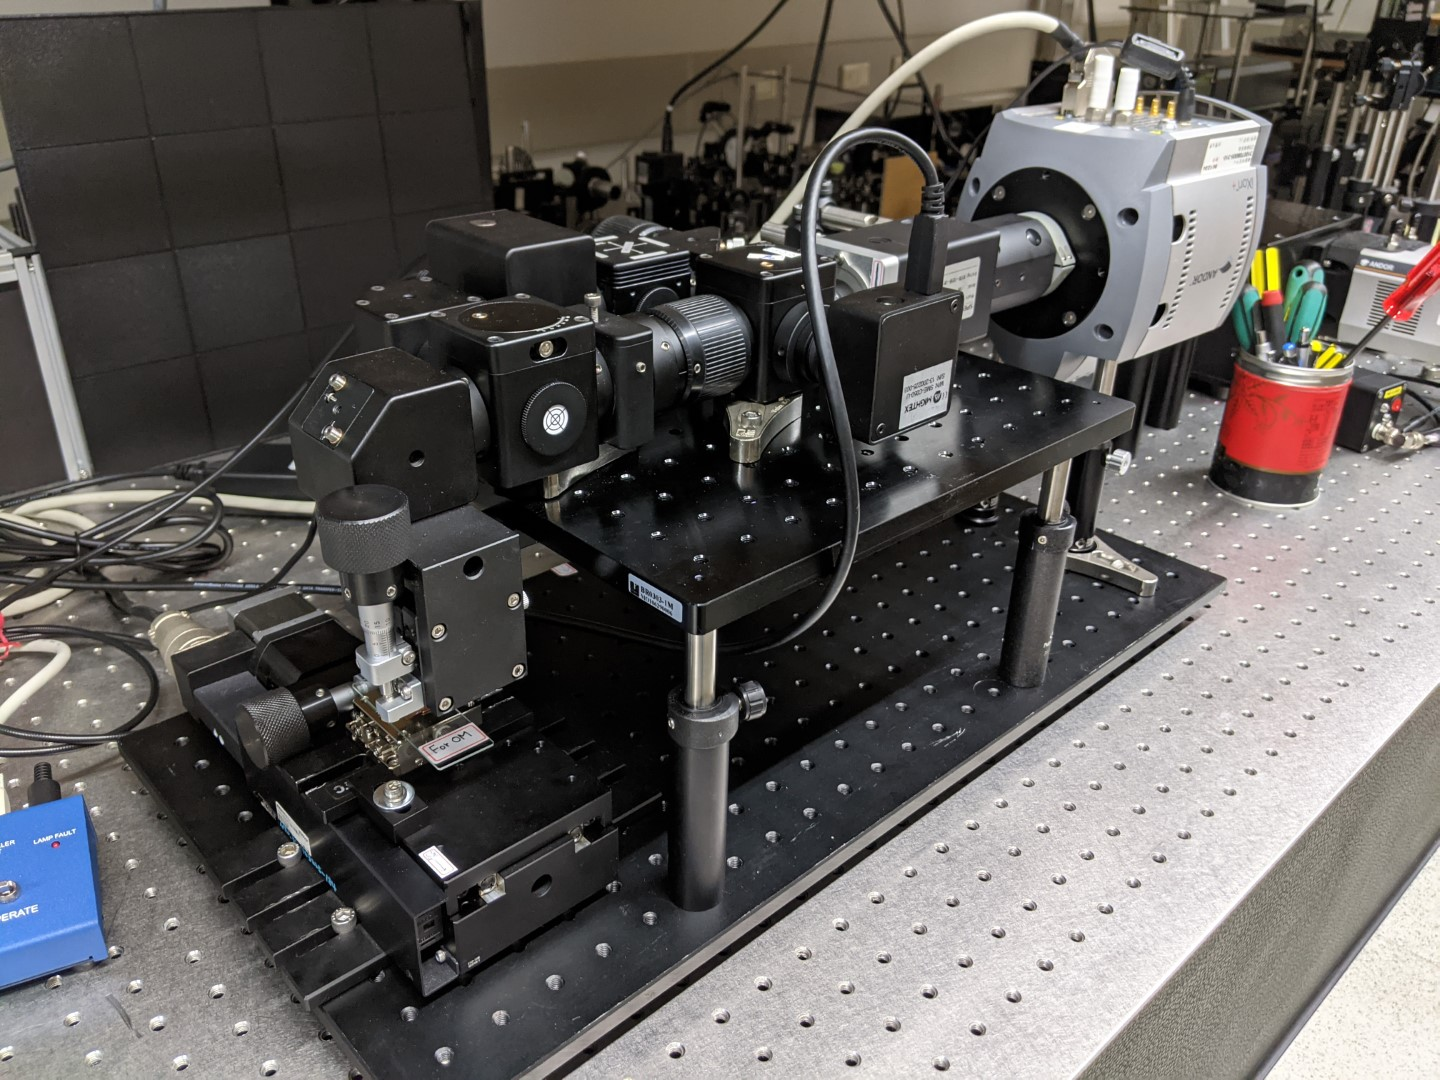
\includegraphics[width=\linewidth]{microSystemPixel3.jpg}
        \end{column}
    \end{columns}
\end{frame}

\subsection{IoT Farm Feild Pest Monitoring Device}
\begin{frame}
    \frametitle{IoT Farm Feild Pest Monitoring Device}
    \begin{columns}
        \begin{column}{0.5\linewidth}
            \begin{itemize}
                \item A self-directed project. May 2020 - present, @Bio-Electromagnetics Lab, NTU
                \item Design a IoT-connected machine to monitor the amount of bugs in farm fields with \href{https://bencer3283.github.io/experiences/Iot/}{\underline{self-designed}} controller board and mechanics.
            \end{itemize}
        \end{column}
        \begin{column}{0.5\linewidth}
            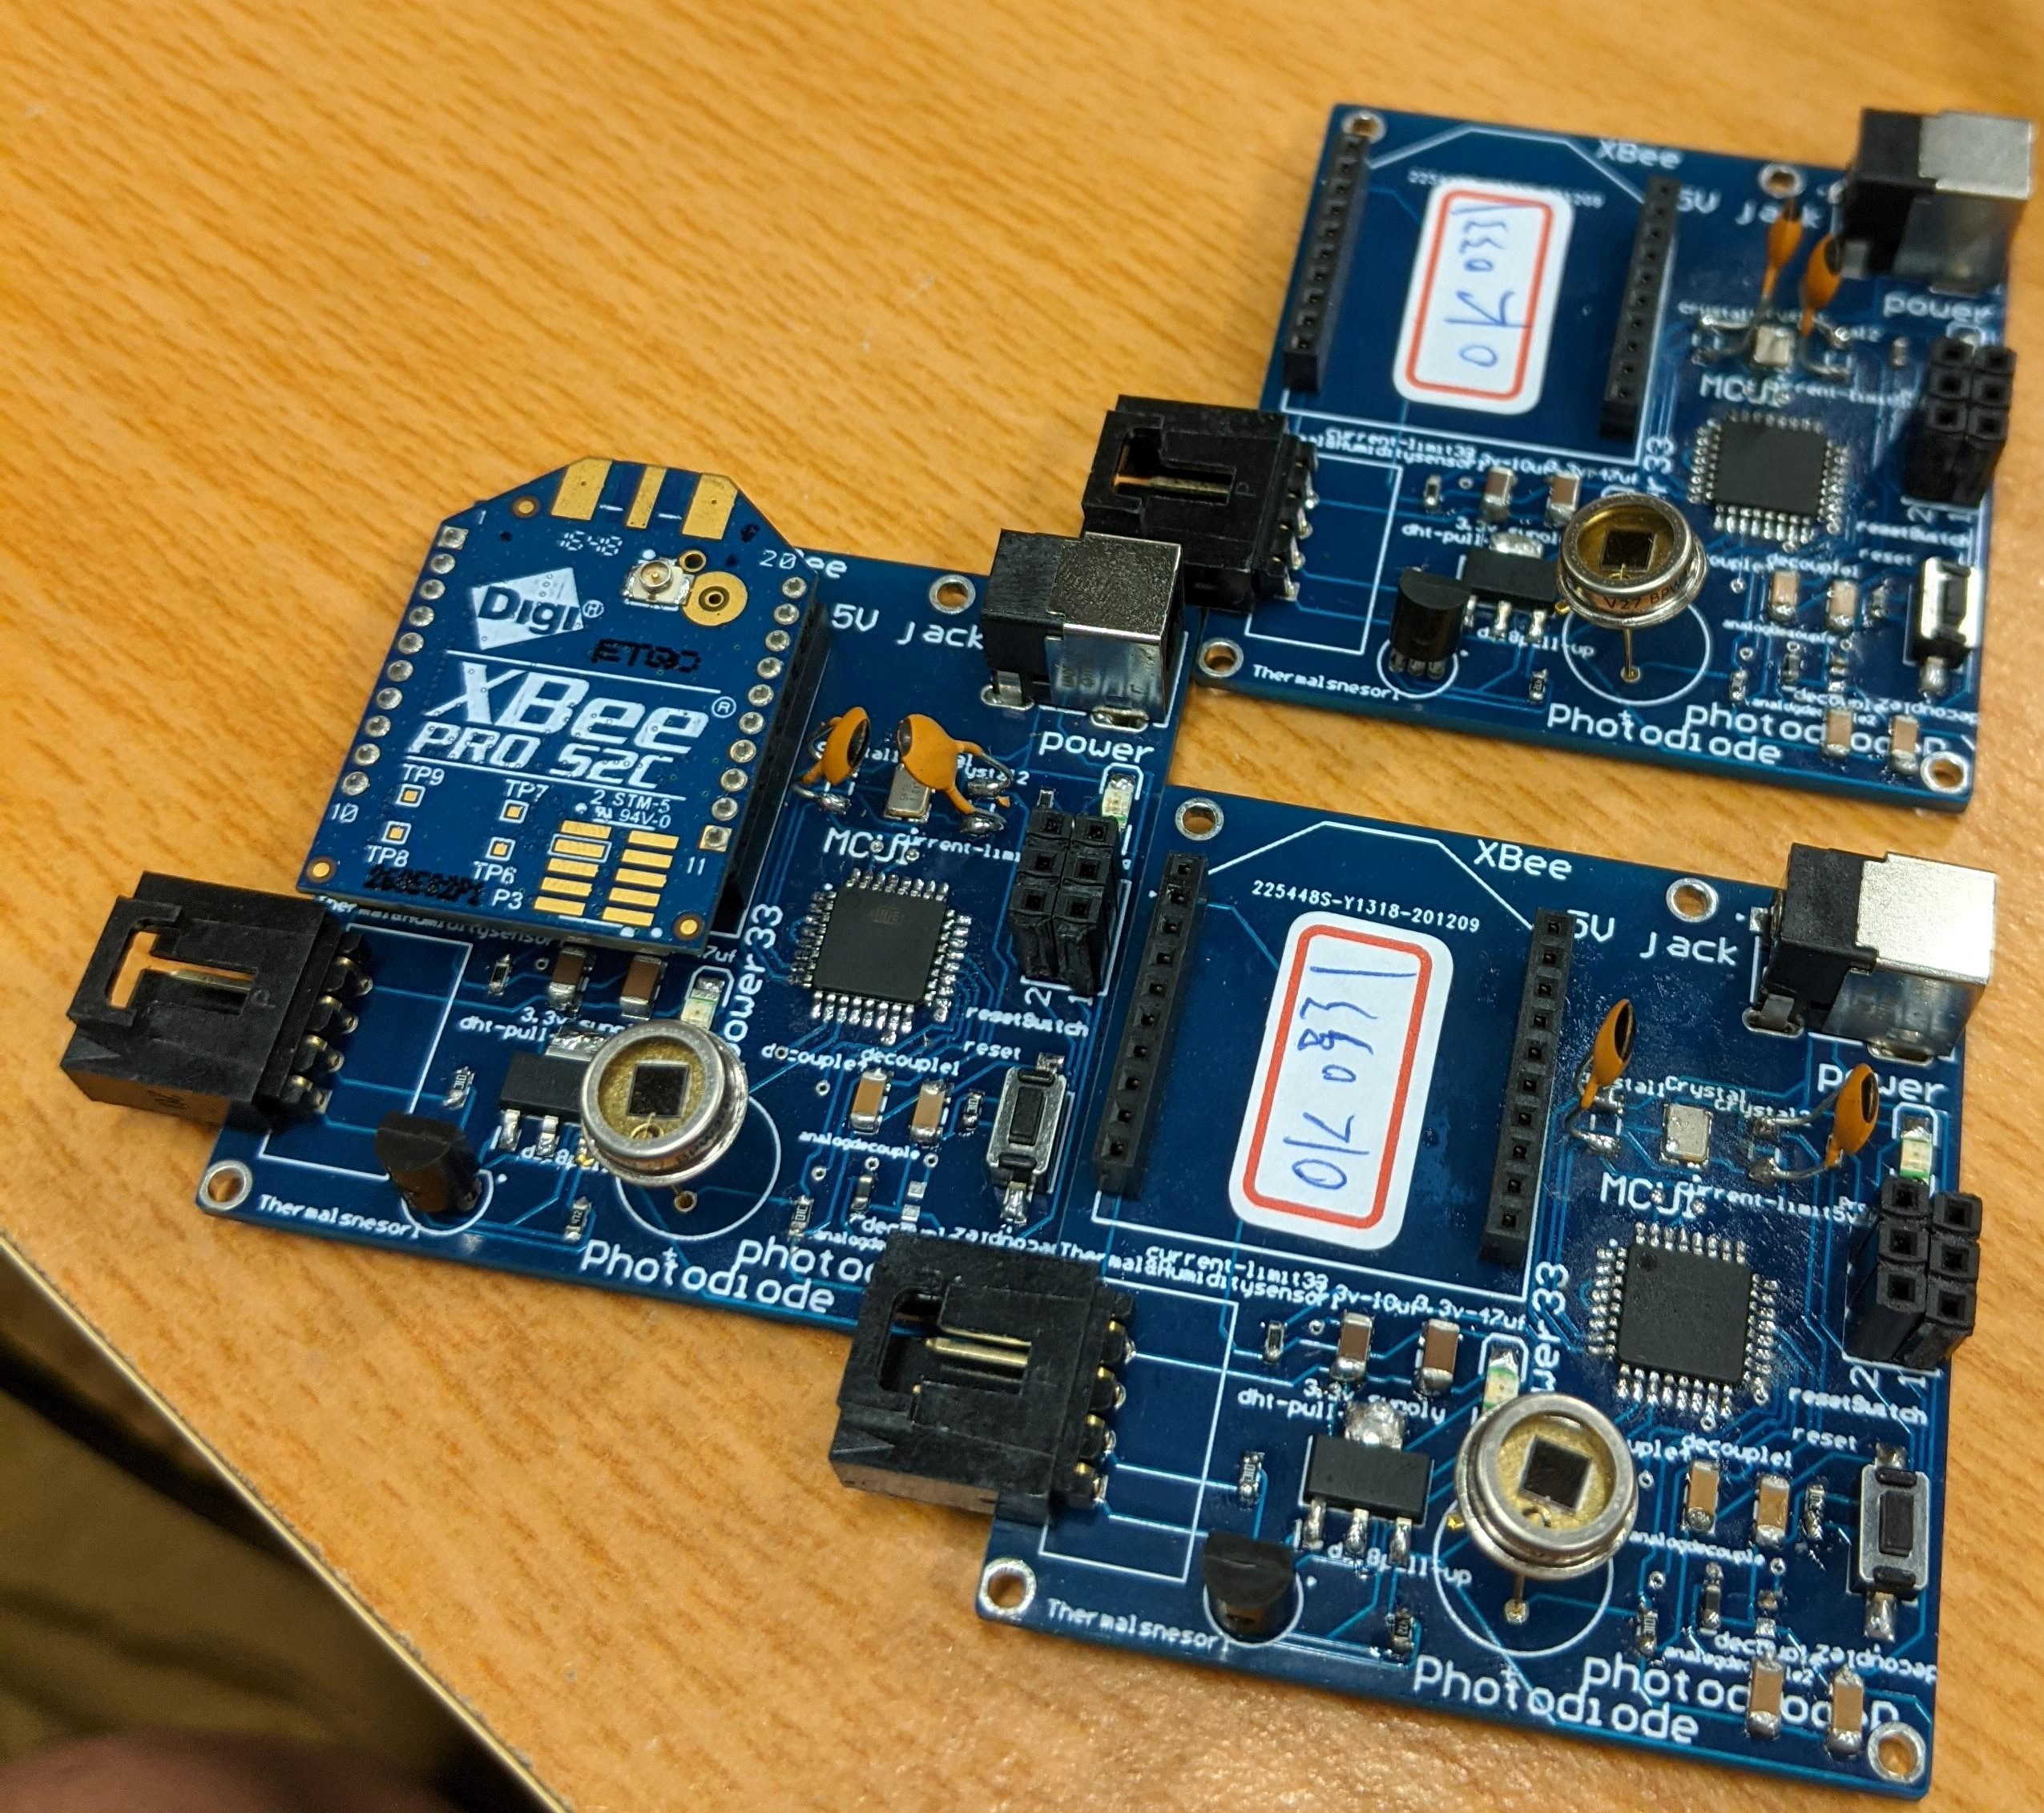
\includegraphics[width=\linewidth]{3pGto7b.jpg}
        \end{column}
    \end{columns}
\end{frame}

\begin{frame}
    \begin{columns}
        \begin{column}{0.5\linewidth}
            \begin{itemize}
                \item Involves mechatronics, IoT (XBee), PCB design (Altium), Python, SolidWorks, microprocessor, Raspberry Pi, MySQL.
            \end{itemize}
        \end{column}
        \begin{column}{0.5\linewidth}
            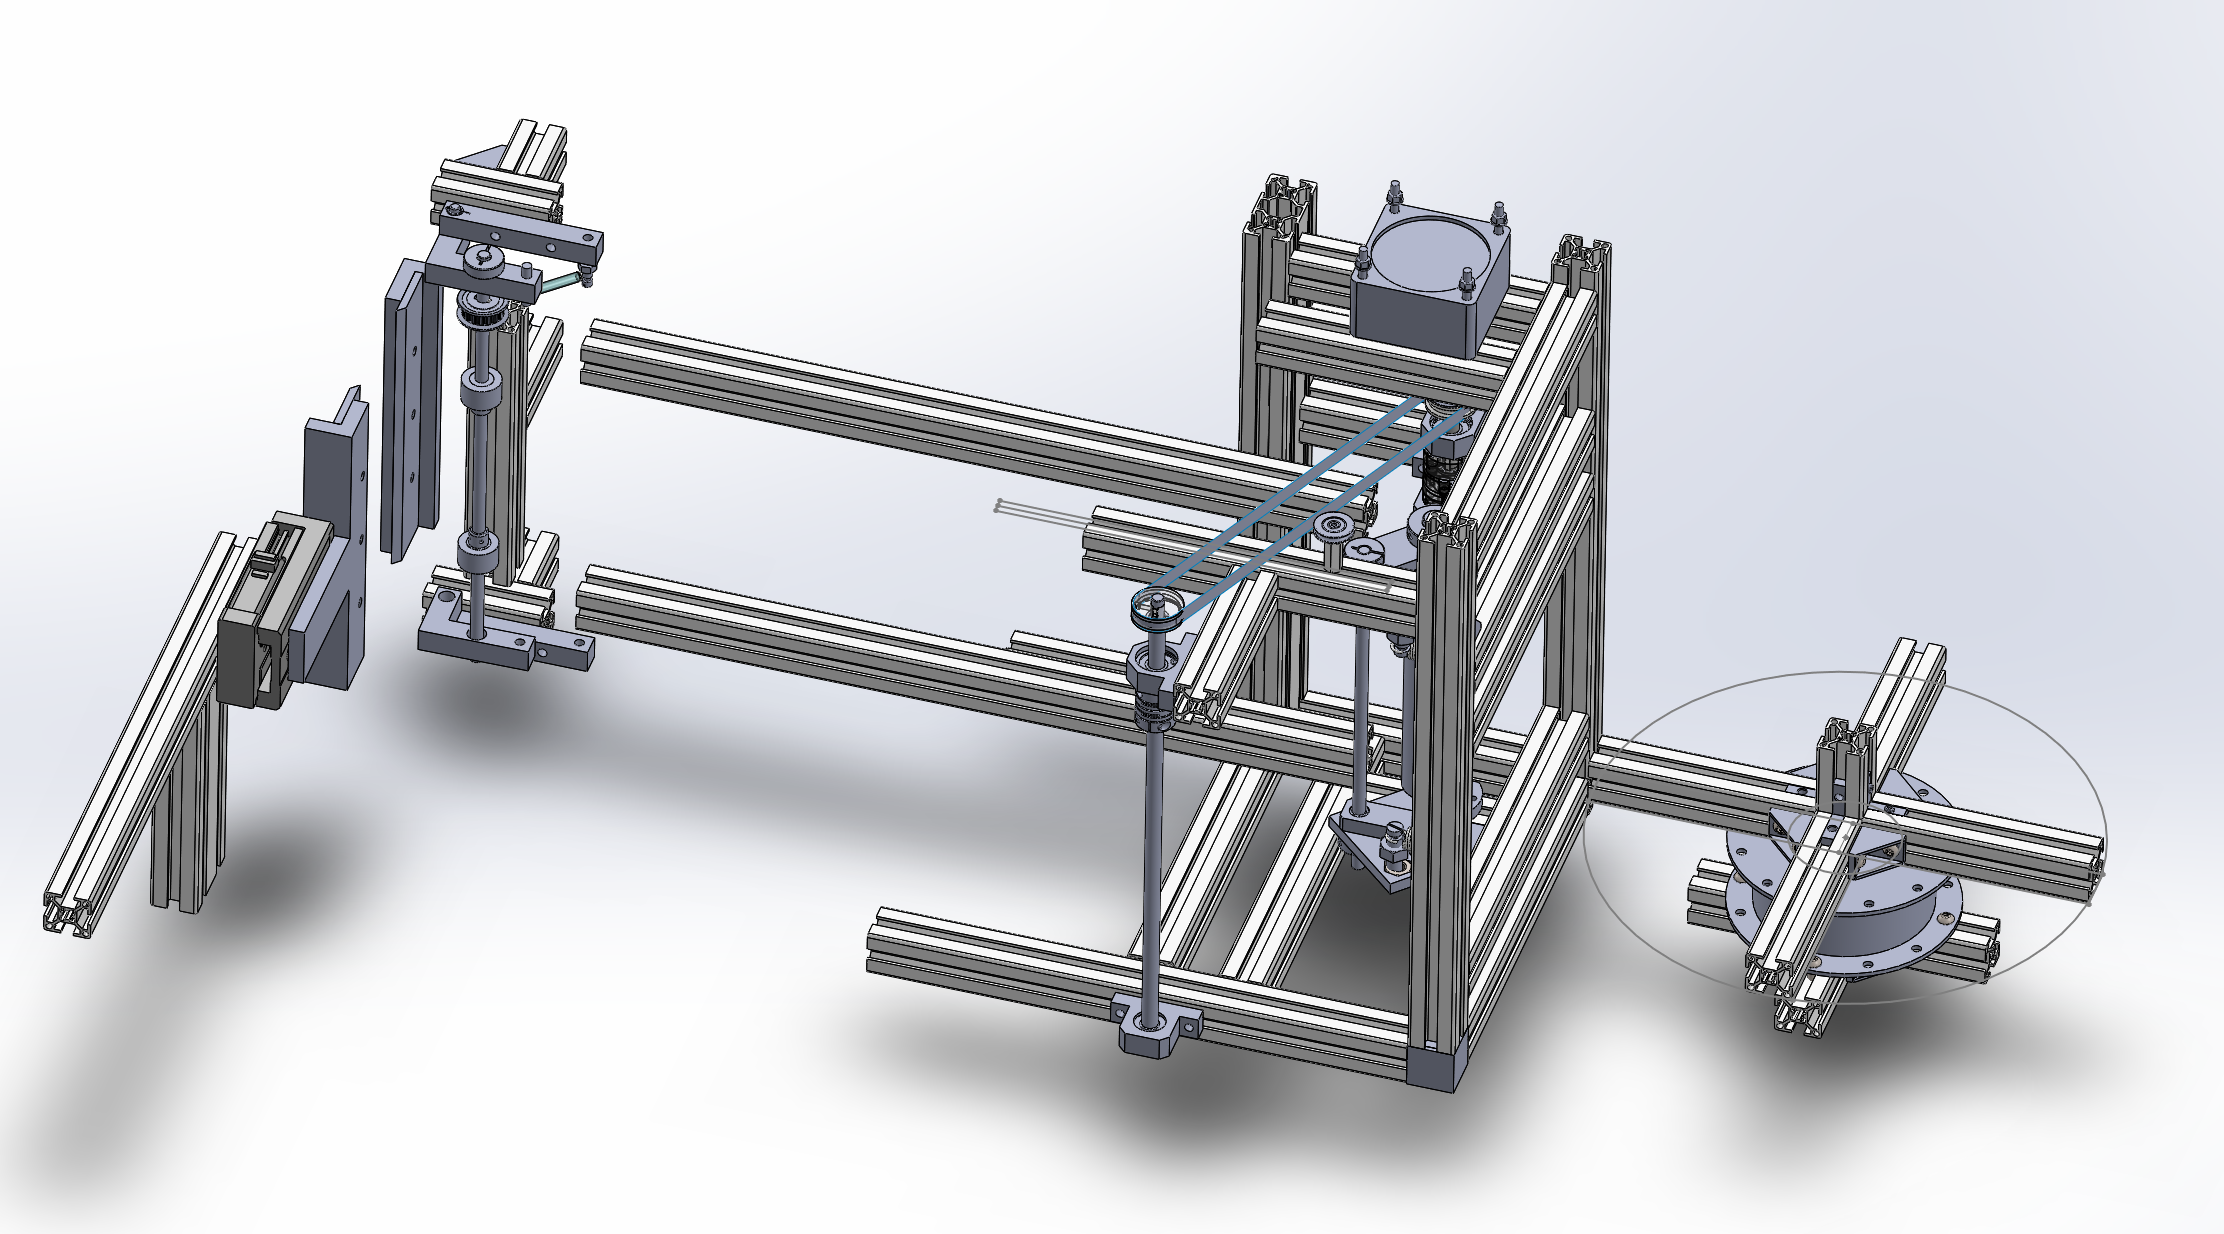
\includegraphics[width=\linewidth]{pestMachine.png}
        \end{column}
    \end{columns}
\end{frame}

\subsection{Golden medalist, 19th Mobileheroes Award}
\begin{frame}
    \frametitle{Golden medalist, 19th Mobileheroes Award}
    \begin{itemize}
        \item Category of 5G innovative application, (NT300,000) awarded by Industrial Development Bureau.
        \item Our team ARGO has developed a AR platform that utilize advanced image-based spacial recognition algorithm that enables complex AR experiences on personal mobile devices.
        \item My main contribution are UI/UX evaluation and design of the AR world for demo.
    \end{itemize}
\end{frame}

\subsection{Championship Thesis on Industrial Impact of COVID}
\begin{frame}
    \frametitle{Championship, 2021 National Thesis Competition for College Students}
    \begin{itemize}
        \item "Covid-19's Impact on Online Video Streaming Platform from The Perspective of Consumer Preference"
        \item In this work we found that most consumers didn't think the pandemic makes than more prone to subscription video services. By our statistics analysis, we found that only "family plan", which reduces price substentially, can make consumers prefer subscription OTT platform.
        \item Involves Matlab for statistics (Chi-square test for independence,
              Logistic regression).
    \end{itemize}
\end{frame}




\section{Strength \& Goals}
\begin{frame}
    \frametitle{NPI}
    % \begin{columns}
    %     \begin{column}{0.25\linewidth}
            \begin{itemize}
                \item Bring it to life
                \item Make or break?
                     Feasibility,
                     viability,
                     desirability,
            \end{itemize}
        % \end{column}
        % \begin{column}{0.75\linewidth}
            \begin{figure}
        \centering
        \includegraphics[width=0.8\textwidth]{npi.jpg}
        \caption{(TCGen, 2023)}
    \end{figure}
    %     \end{column}
    % \end{columns}
    
\end{frame}

\begin{frame}
    \frametitle{Good at everything. Good at nothing.}
    \begin{itemize}
        \item Design + Engineering Prototyping
        \begin{itemize}
            \item CAD + 3D Printing
            \item Industrial Automation + Mechanics
            \item Embedded Computing + Circuits
            \item Software Development
        \end{itemize}
    \end{itemize}
\end{frame}


\end{document}